\documentclass[9pt]{article}
\usepackage{blindtext}
\usepackage{multicol}
\usepackage{mathptmx}
\usepackage{graphicx}

\setlength{\columnsep}{0.5cm}


\title{\textbf{\LARGE{Step Prediction Regulating Method to Increase the Reliability of PID Controllers}}}
\author{\Large{Gokhan Tekir }}
\date{April 2021}

\usepackage{geometry}
 \geometry{
 a4paper,
 left=20mm,
 right=20mm,
 top=25mm,
 bottom=37mm
 }
 
\begin{document}
\maketitle

\section{Abstract}
\textbf{Complicated systems that needs to work as efficient as possible or the simple systems that needs to do complicated tasks with maximum efficiency needs a lot of effort and mathematics. To make a system reliable; adding more control algorithms to system makes the system unreliable because every control algorithm has their own tuning constants and using methods.
This article aims to increase reliability of PID Controllers by a new method called Step Prediction Regulating.}


\section{Introduction}
\begin{multicols}{2}
A control system is a combination of components 
that regulates the behavior of other devices or systems 
to produce the desired output. 
So many control algorithms depend on mathematical models of 
dynamical systems to describe the system dynamics accurately and deterministically. 
However, parameters and/or conditions of dynamical systems may not be always determined exactly[1].Despite the advent of many sophisticated
control theories and techniques, the majority of
industrial processes nowadays are still regulated
by PID controllers[2].The PID controller is thus the bread and butter of automatic
control.It is the first solution that should be tried when
feedback is used[3]. PID control is by far the dominating control
structure in industrial practice[4].
The birth and large-scale deployments of the powerful yet primitive proportional–integral–derivative (PID) control law dates back to the period of the 1920s–1940s in the last century, in response to the pressing demands of industrial
automation before, during, and particularly after World War II[5].\\[0.4mm]
Proportional integral derivative (PID) controllers are widely used in the process control industry, the main reason is its relatively simple structure, which can be easily understood and implemented in practice[6]. With its three-term functionality offering treatment of both transient and steady-state responses, proportional-integral-derivative (PID) control provides a generic and efficient solution to realworld control problems[7]. Conventional proportional–integral–derivative (PID)
controllers have been well developed and applied for
about half a century, and are extensively used for industrial
automation and process control today[8]. Proportional integral derivative (PID) controllers are still widely used in the process industries even though control
theory has been developed significantly since they were
first used decades ago[9].\\[0.4mm]
PID controller takes 3 different constant numbers(excluding fuzzy systems).
These numbers took their name after the processes they go through. PID controllers are commonly used in practice in the process control industries. They can be tuned by using rules of thumb (Ziegler and Nichols, 1942) or formulae
resulting from analytical design (AsstroKm and HaKgglund,1984)[10].\\[0.4mm]
There is also another powerfull control algorithm. The MPC(Model Predictive Control). More than 15 years after model predictive control (MPC) appeared in industry as an effective means to deal with multivariable constrained control problems, a theoretical basis for this technique has started to emerge[11].\\[0.4mm]
Model Predictive Control (MPC), also referred to as Receding Horizon Control and Moving Horizon Optimal Control, has been widely adopted in industry as an effective means to deal with multivariable constrained control problems[12].\\[0.4mm]
Model predictive control (MPC) refers to a class of
computer control algorithms that utilize an explicit
process model to predict the future response of a plant.[13]
Academic researchers have investigated so many theoretical aspects of MPC that
it is a staple ingredient of innumerable journal and conference papers, and monographs.[14]\\[0.4mm]
But there is also another problem named dead-time problem that hasn't solved yet.
Dead-time is the time between the steps of the system that system can't react. The most popular solution for this specific problem is the Smith Predictor.\\[0.4mm]
In the late 1950s, 0. J. M. Smith proposed a controller
that became known as a Smith Predictor. He first suggested
this control scheme for factory processes with long transport delays, for example catalytic crackers and steel mills
(Smith, 1959). but the idea can be generalized to all control
processes that have long loop delays[15]. The Smith predictor is a popular and very effective long dead-time compensator for stable processes.[16-17]\\[0.4mm]
A CLASSICAL problem of control theory is that of
synthesizing controllers which regulate systems
despite uncertainty in plant and controller
parameters[18].

\section{Methods}
There are too many uncertainties to calculate to make a real-life system work as efficiently as possible; like static and dynamic friction, air pressure, the efficiency of the components; external influences such  as an impact, an object standing in front of the system. These uncertainties make the system unreliable and 
inefficient. This problems can be avoid by using Step Prediction Regulating method.\\[0.4mm]
Step prediction regulating method works very similar to smith predictors. But instead of dealing with the dead-time
problem. Step prediction regulating method deals with external errors. This method can be referred as the combination of PID, MPC controllers and Smith Predictors.\\[0.4mm]
Step prediction regulating involves 2 parts as step prediction and regulating. This two parts has 2 differrent jobs and they are individually important. Step prediction part behaves like MPC controllers because it predicts the future. But instead of fitting up the model to a dataset, this part actually creates another algorithm that doesn't include real life external errors. So far, the system has two individual controller outputs. One works like a trajectory planner and the other one is for following the first one.\\[0.4mm]
PID Controller equation:

\begin{equation}
    \scalebox{0.85}{$K_p \times e(t) + K_i \times \int_{0}^{t} e(t)\times dt + K_d \times\frac{de}{dt}$}
\end{equation}
\\[0.4mm]
The math behind Step Prediction method works a bit differently. As mentioned before, Step Prediction method has two different controllers.\\[0.4mm]
The controller has no external errors in it:\\[0.4mm]
\begin{equation}
\scalebox{0.85}{$
g(e) = \int_{(m-1)\times K_{loop}}^{K_{loop}\times m} K_p\times e(t) + K_i\times \int_{t\times(m-1)}^{K_{loop}\times m} e(n)\times dt + K_d \times \frac{de}{dt}\times dt$}
\end{equation}\\[0.4mm]
As can be seen from the equation above, there is a lot of variables in it. $e$ stands for the error, $K_{loop}$ stands for the $Prediction Horizon$. $Prediction Horizon$ is the value that represents how much will the system predicts to future. This will
be determined by the user of the system. Lastly, $m$ stands for index numbers of the $K_{loop}$. The $m$ values job is to split the predictions into $K_{loop}$ sized steps.\\[0.4mm]
The controller has external errors in it:\\[0.4mm]
\begin{equation}
    \scalebox{0.85}{$f(e) = g(e) - external_{errors}$}
\end{equation}\\[0.4mm]
As can bee seen from the second equation, the only difference between these two controller is the external errors. External errors will create the differences between two controllers. Thus, the Regulating Controller can follow the Prediction Controller. This difference plays a big role in Step Prediction method.\\[0.4mm]
Storing both of the controllers to create the data for rho function:\\[0.4mm]
\begin{equation}
    \scalebox{0.85}{$G = [ g(n),g(n+1)\dots,g(K_{loop})]$}
\end{equation}
\begin{equation}
    \scalebox{0.85}{$F = [ f(n),f(n+1)\dots,f(K_{loop})]$}
\end{equation}\\[0.4mm]
Stored data will create the function named rho function. Rho function calculates the output difference between planned trajectory(first equation) and
real world outputs(second equation) to determine how much to increase the output for each step.\\[0.4mm]
Rho function:\\[0.4mm]
\begin{equation}
    \scalebox{0.85}{$\rho(e) = \frac{F_{(m-1) \times K_{loop}} - G_{m\times K_{loop}}}{dt}$}
\end{equation}\\[0.4mm]
The final equation is the combination of all of the equations above.\\[0.4mm]
Step Prediction function:\\[0.4mm]
\begin{equation}
 \scalebox{0.85}{$h(e) = \int_{(m-1)\times K_{loop}}^{K_{loop}\times m} K_p\times e(t) + K_i\times \int_{t\times(m-1)}^{K_{loop}\times m} e(n)\times dt + K_d \times \frac{de}{dt}\times dt + K_{\rho} \times \rho(e)$}
\end{equation}\\[0.4mm]
With the addition of $K_{\rho}$ and $\rho(e)$ parts, controller will be able to increase the output for every step to reach the planned trajectory that planned by Prediction Controller.\\[0.4mm]
To simulate all the different aspects of this controller there will be 20 different simulations the difference between these simulations is the tuning differences.\\[0.4mm]
\end{multicols}
\section{Results}
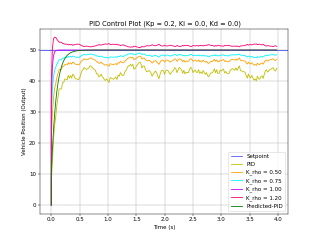
\includegraphics[scale=.425]{figures/Figure_1.png}
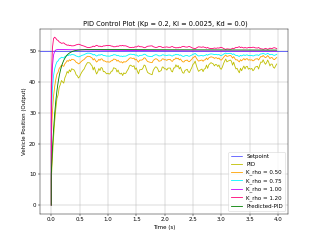
\includegraphics[scale=.425]{figures/Figure_2.png}\\[0.4mm]
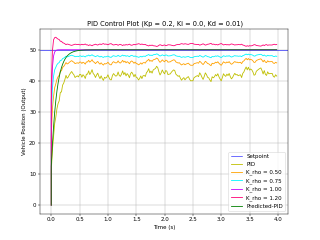
\includegraphics[scale=.425]{figures/Figure_3.png}
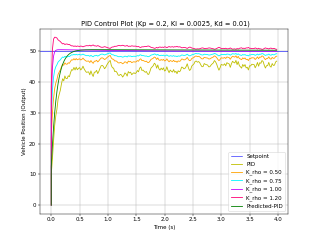
\includegraphics[scale=.425]{figures/Figure_4.png}

\section{Discussion}

When it comes to designing control algorithms, its hard to predict the differences between simulated outputs and real world outputs. Using step prediction regulating method can require hard work for creating and tuning for a specific system. However, step prediction regulating method is designed for solving such problems.

When $Rho_d$ constant goes to 1, the difference between trajectory controller and real-world controller nearly goes to 0. When that happens, system makes some hard turns which makes the system unreliable,
When $Rho_d$ constant is "0.5" the $\rho e$ controller becomes insufficient. In conclusion, with a proper tuning, Step Prediction Controller method can make differences.
\pagebreak

\section{References}

1) Najariyan,M.,Zhao, Y.(2020).Granular fuzzy PID controller. Expert Systems with Applications, 114182.\newline2)  He, S.-Z., Tan, S., Xu, F.-L., and Wang, P.-Z. (1993). Fuzzy self-tuning of PID controllers. Fuzzy Sets and Systems, 56(1), 37–46.\newline3) Åström, K. J., Hägglund, T. (2001). The future of PID control. Control Engineering Practice, 9(11), 1163–1175.\newline4) Åarzén, K.-E. (1999). A simple event-based PID controller. IFAC Proceedings Volumes, 32(2), 8687–8692\newline5) Han, J. (2009). From PID to Active Disturbance Rejection Control. IEEE Transactions on Industrial Electronics, 56(3), 900–906.\newline6) Qing-Guo Wang, Tong-Heng Lee, Ho-Wang Fung, Qiang Bi, and Yu Zhang. (1999). PID tuning for improved performance. IEEE Transactions on Control Systems Technology, 7(4), 457–465.\newline7) PID control system analysis and design. (2006). IEEE Control Systems, 26(1), 32–41.\newline8) Tang, K. S., Kim Fung Man, Guanrong Chen, Kwong, S. (2001). An optimal fuzzy PID controller. IEEE Transactions on Industrial Electronics, 48(4), 757–765\newline9) Zhuang, M., and Atherton, D. P. (1993). Automatic tuning of optimum PID controllers. IEE Proceedings D Control Theory and Applications, 140(3)\newline10) Majhi, S., and Atherton, D. P. (2000). Obtaining controller parameters for a new Smith predictor using autotuning. Automatica, 36(11), 1651–1658.\newline11) Morari, M., H. Lee, J. (1999). Model predictive control: past, present and future. Computers and Chemical Engineering, 23(4-5), 667–682.\newline12) Bemporad, A., and Morari, M. (n.d.). Robust model predictive control: A survey. Lecture Notes in Control and Information Sciences, 207–226.\newline13) Qin, S. J., and Badgwell, T. A. (2003). A survey of industrial model predictive control technology. Control Engineering Practice, 11(7), 733–764.\newline14) Kouvaritakis, B., and Cannon, M. (2016). Model Predictive Control. Advanced Textbooks in Control and Signal Processing.\newline15) Miall, R. C., Weir, D. J., Wolpert, D. M., and Stein, J. F. (1993). Is the Cerebellum a Smith Predictor? Journal of Motor Behavior, 25(3), 203–216.\newline16) Astrom, K. J., Hang, C. C., and Lim, B. C. (1994). A new Smith predictor for controlling a process with an integrator and long dead-time. IEEE Transactions on Automatic Control, 39(2), 343–345.\newline17) S.Majhi and D.P.Atherton(1999). Modified Smith predictor and controller for processes with time delay\newline18) Francis, B. A.,Wonham, W. M. (1976). The internal model principle of control theory. Automatica, 12(5), 457–465. 

\end{document}
